\section{\result}
\begin{figure}[H]
    \centering
    \begin{minipage}[b]{.49\columnwidth}
        \centering
        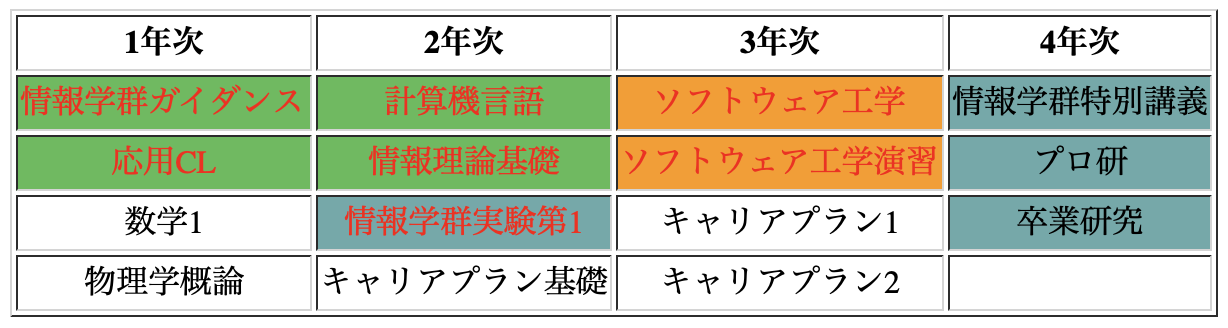
\includegraphics[keepaspectratio,width=\textwidth]{../../10_UniversalDesign/no1_table_original.png}
        \subcaption{改良前(C型)}
    \end{minipage}
    \begin{minipage}[b]{.49\columnwidth}
        \centering
        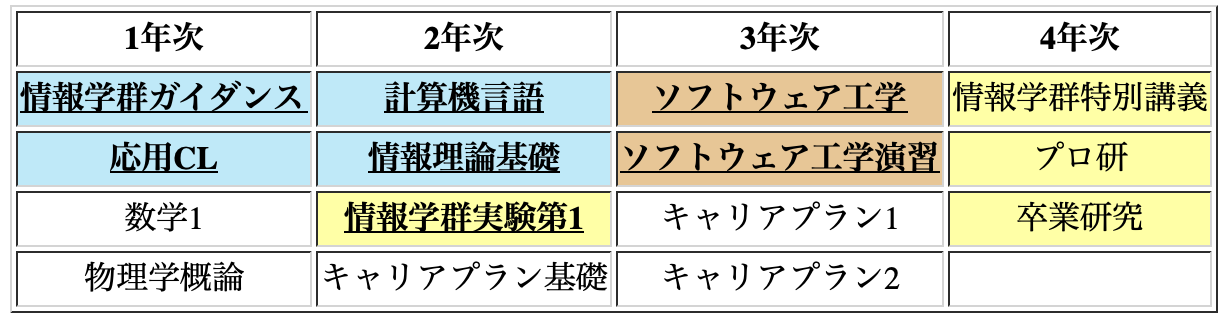
\includegraphics[keepaspectratio,width=\textwidth]{../../10_UniversalDesign/no1_tableR_original.png}
        \subcaption{改良後(C型)}
    \end{minipage}
    \begin{minipage}[b]{.49\columnwidth}
        \centering
        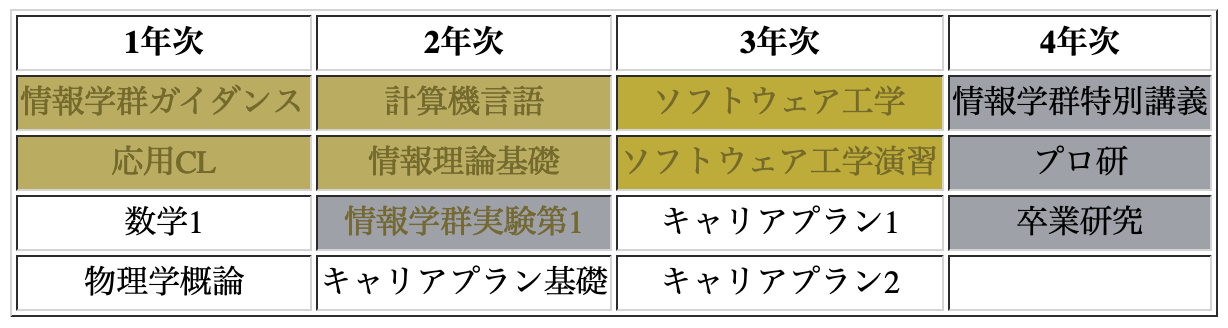
\includegraphics[keepaspectratio,width=\textwidth]{../../10_UniversalDesign/no1_table_OC_P.png}
        \subcaption{改良前(P型)}
    \end{minipage}
    \begin{minipage}[b]{.49\columnwidth}
        \centering
        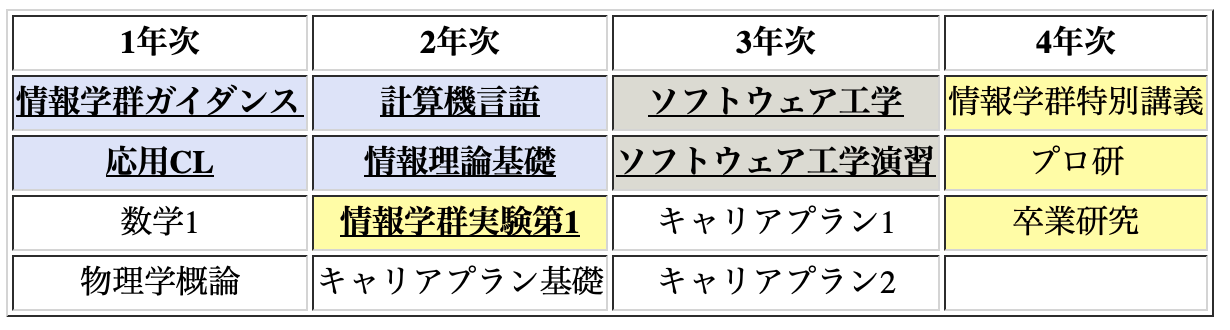
\includegraphics[keepaspectratio,width=\textwidth]{../../10_UniversalDesign/no1_table_RC_P.png}
        \subcaption{改良後(P型)}
    \end{minipage}
    \begin{minipage}[b]{.49\columnwidth}
        \centering
        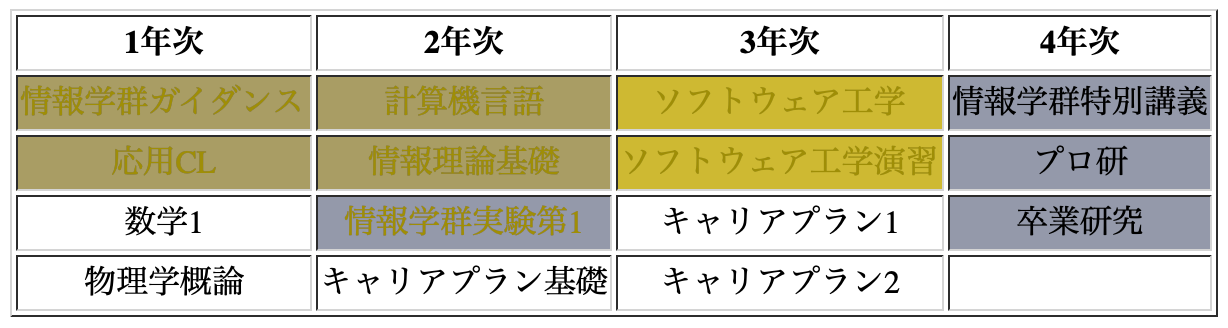
\includegraphics[keepaspectratio,width=\textwidth]{../../10_UniversalDesign/no1_table_OC_D.png}
        \subcaption{改良前(D型)}
    \end{minipage}
    \begin{minipage}[b]{.49\columnwidth}
        \centering
        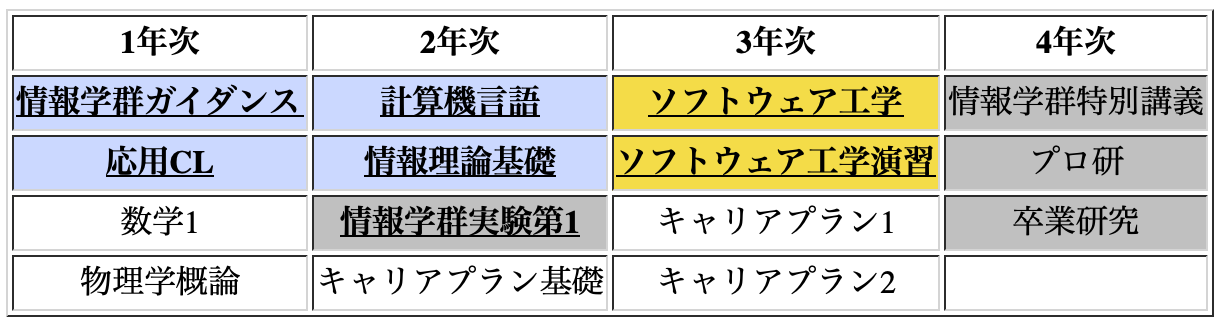
\includegraphics[keepaspectratio,width=\textwidth]{../../10_UniversalDesign/no1_table_RC_D.png}
        \subcaption{改良後(D型)}
    \end{minipage}
    \begin{minipage}[b]{.49\columnwidth}
        \centering
        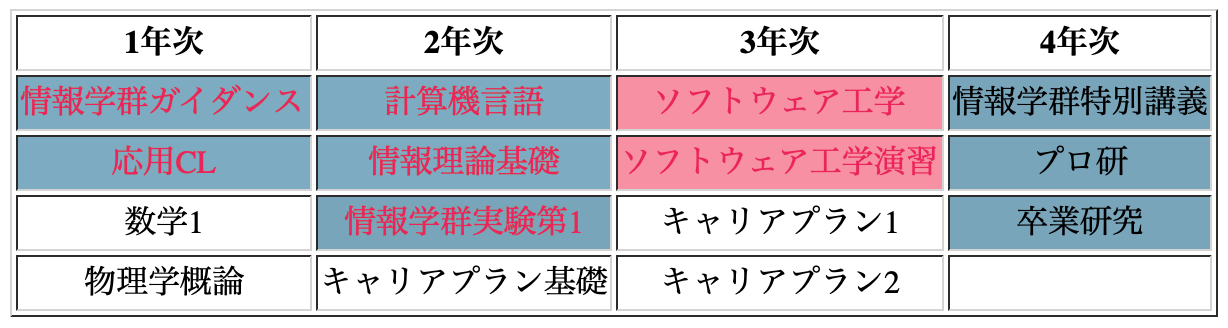
\includegraphics[keepaspectratio,width=\textwidth]{../../10_UniversalDesign/no1_table_OC_T.png}
        \subcaption{改良前(T型)}
    \end{minipage}
    \begin{minipage}[b]{.49\columnwidth}
        \centering
        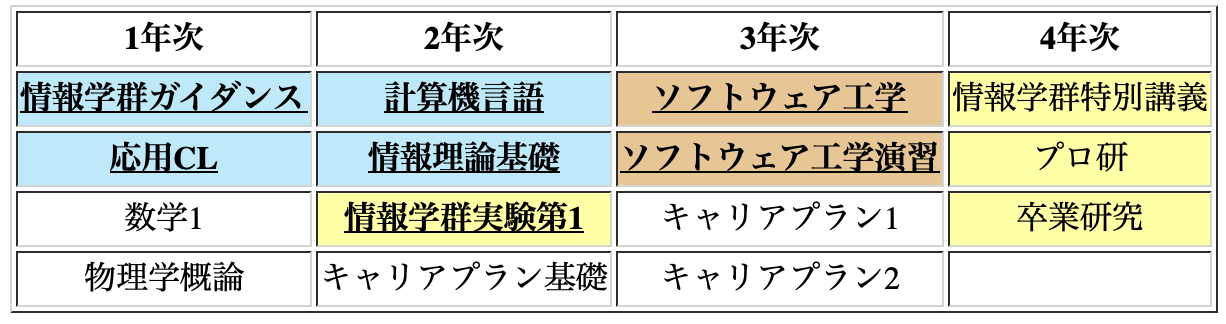
\includegraphics[keepaspectratio,width=\textwidth]{../../10_UniversalDesign/no1_table_RC_T.png}
        \subcaption{改良後(T型)}
    \end{minipage}
    \caption{講義一覧}
\end{figure}
\begin{figure}[H]
    \centering
    \begin{minipage}[b]{.49\columnwidth}
        \centering
        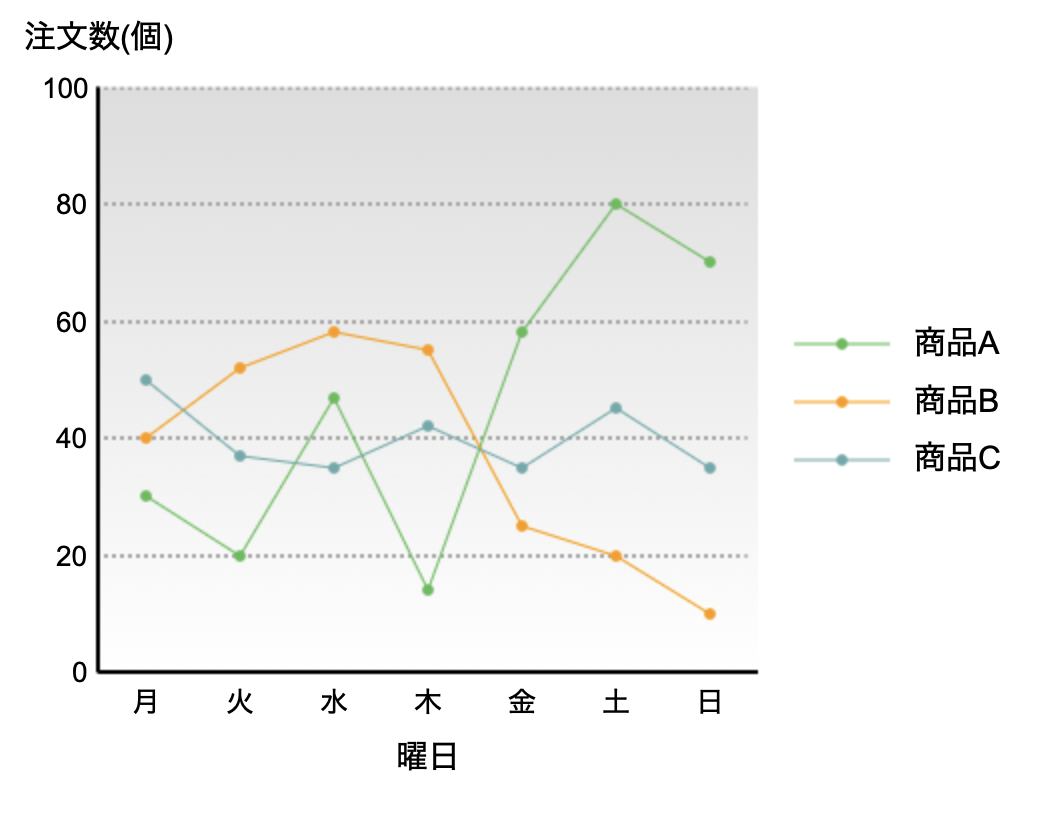
\includegraphics[keepaspectratio,width=\textwidth]{../../10_UniversalDesign/no2_line_original.png}
        \subcaption{改良前(C型)}
    \end{minipage}
    \begin{minipage}[b]{.49\columnwidth}
        \centering
        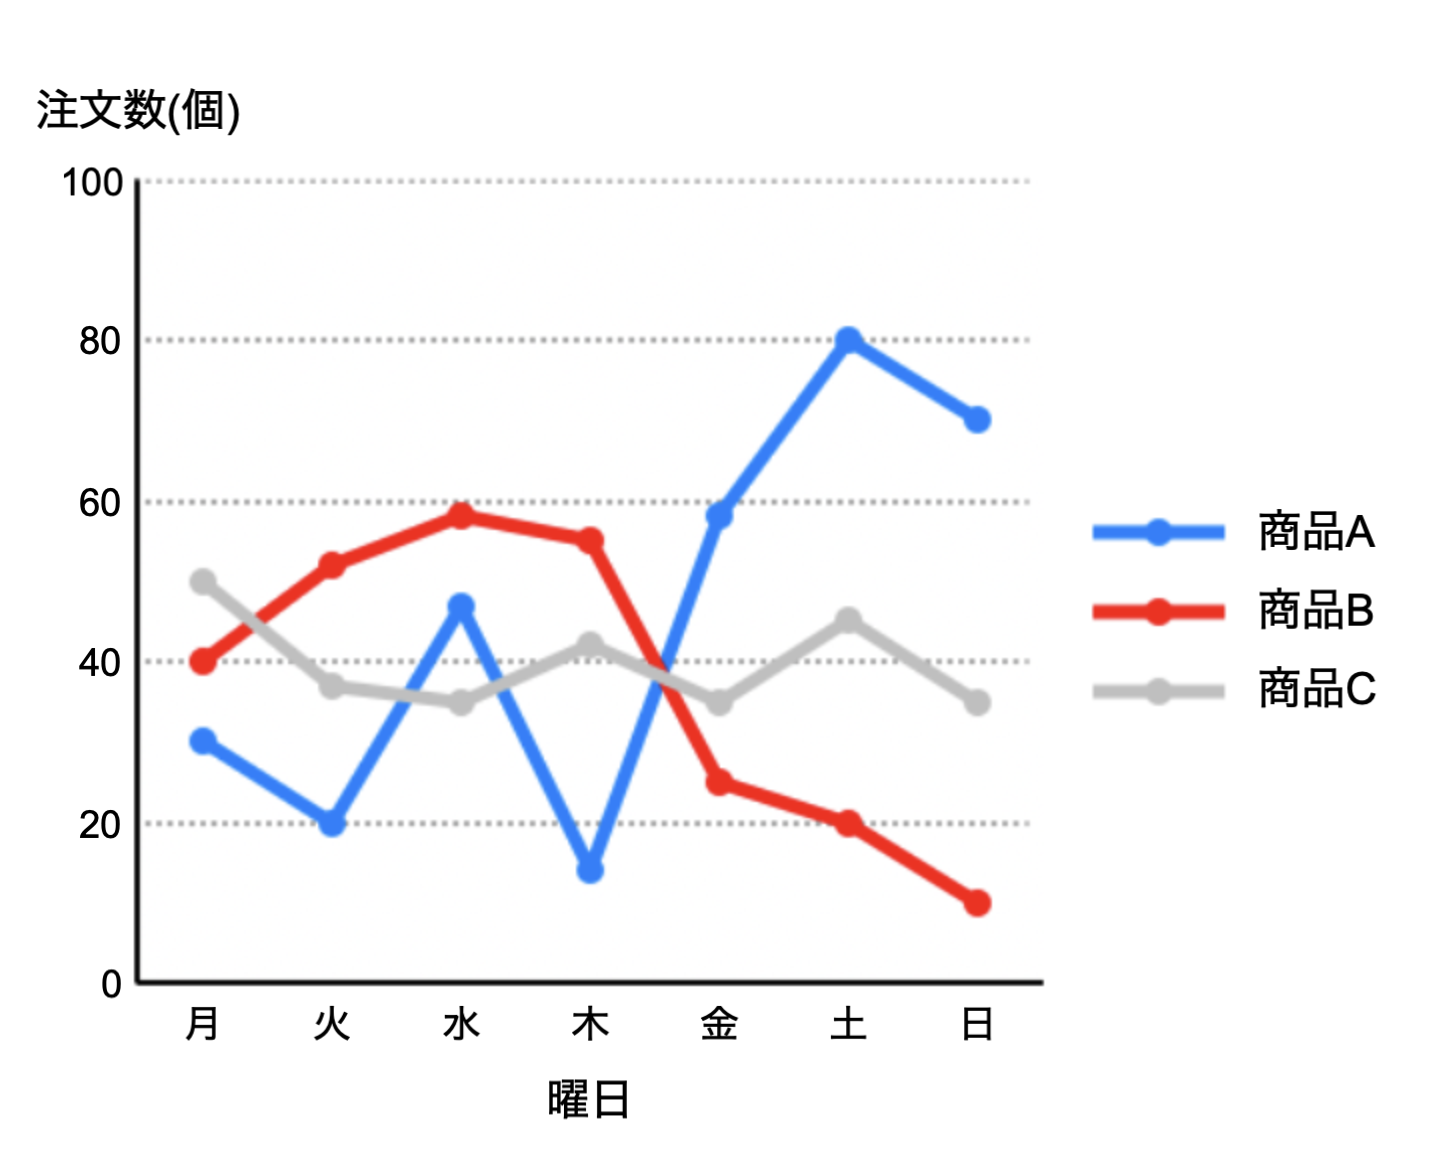
\includegraphics[keepaspectratio,width=\textwidth]{../../10_UniversalDesign/no2_line_reviced.png}
        \subcaption{改良後(C型)}
    \end{minipage}
    \begin{minipage}[b]{.49\columnwidth}
        \centering
        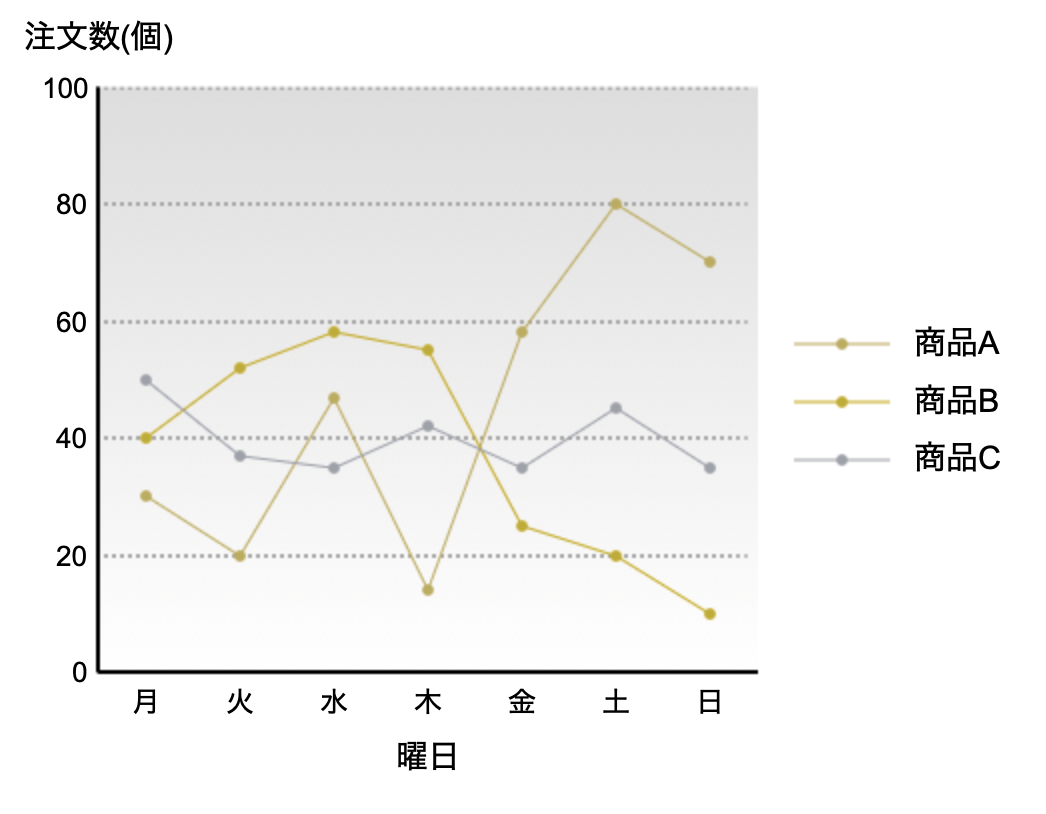
\includegraphics[keepaspectratio,width=\textwidth]{../../10_UniversalDesign/no2_line_CC_P.png}
        \subcaption{改良前(P型)}
    \end{minipage}
    \begin{minipage}[b]{.49\columnwidth}
        \centering
        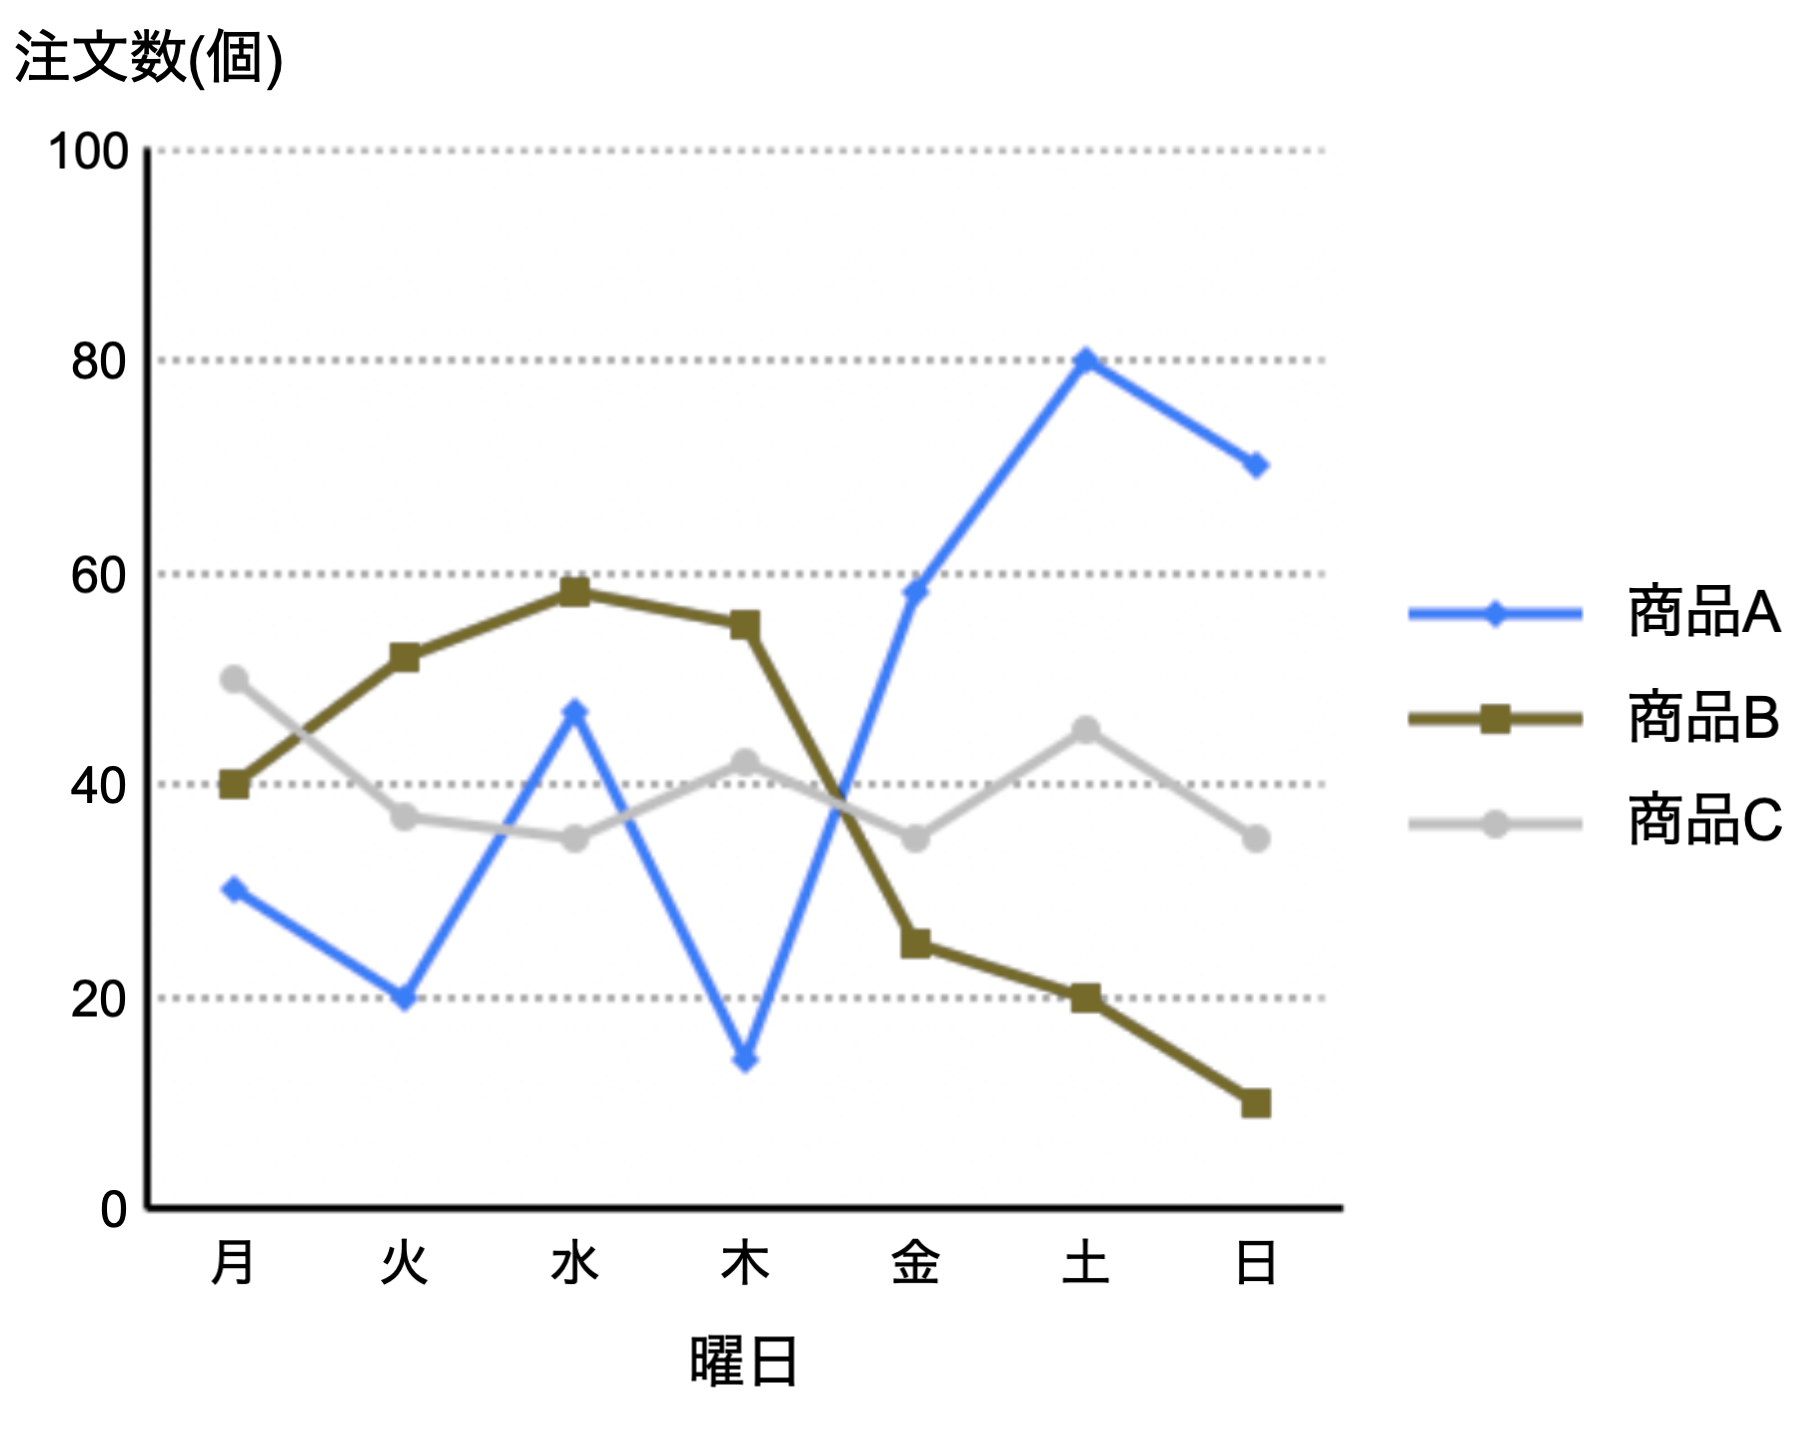
\includegraphics[keepaspectratio,width=\textwidth]{../../10_UniversalDesign/no2_line_RC_P.png}
        \subcaption{改良後(P型)}
    \end{minipage}
    \begin{minipage}[b]{.49\columnwidth}
        \centering
        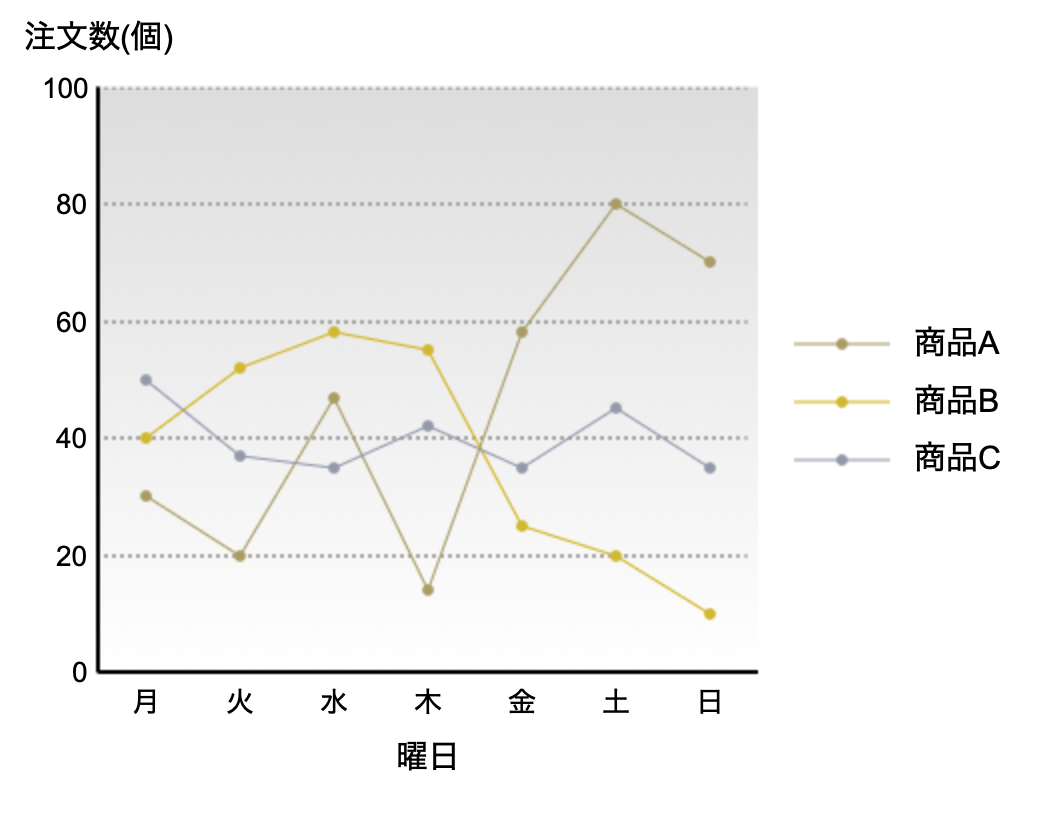
\includegraphics[keepaspectratio,width=\textwidth]{../../10_UniversalDesign/no2_line_CC_D.png}
        \subcaption{改良前(D型)}
    \end{minipage}
    \begin{minipage}[b]{.49\columnwidth}
        \centering
        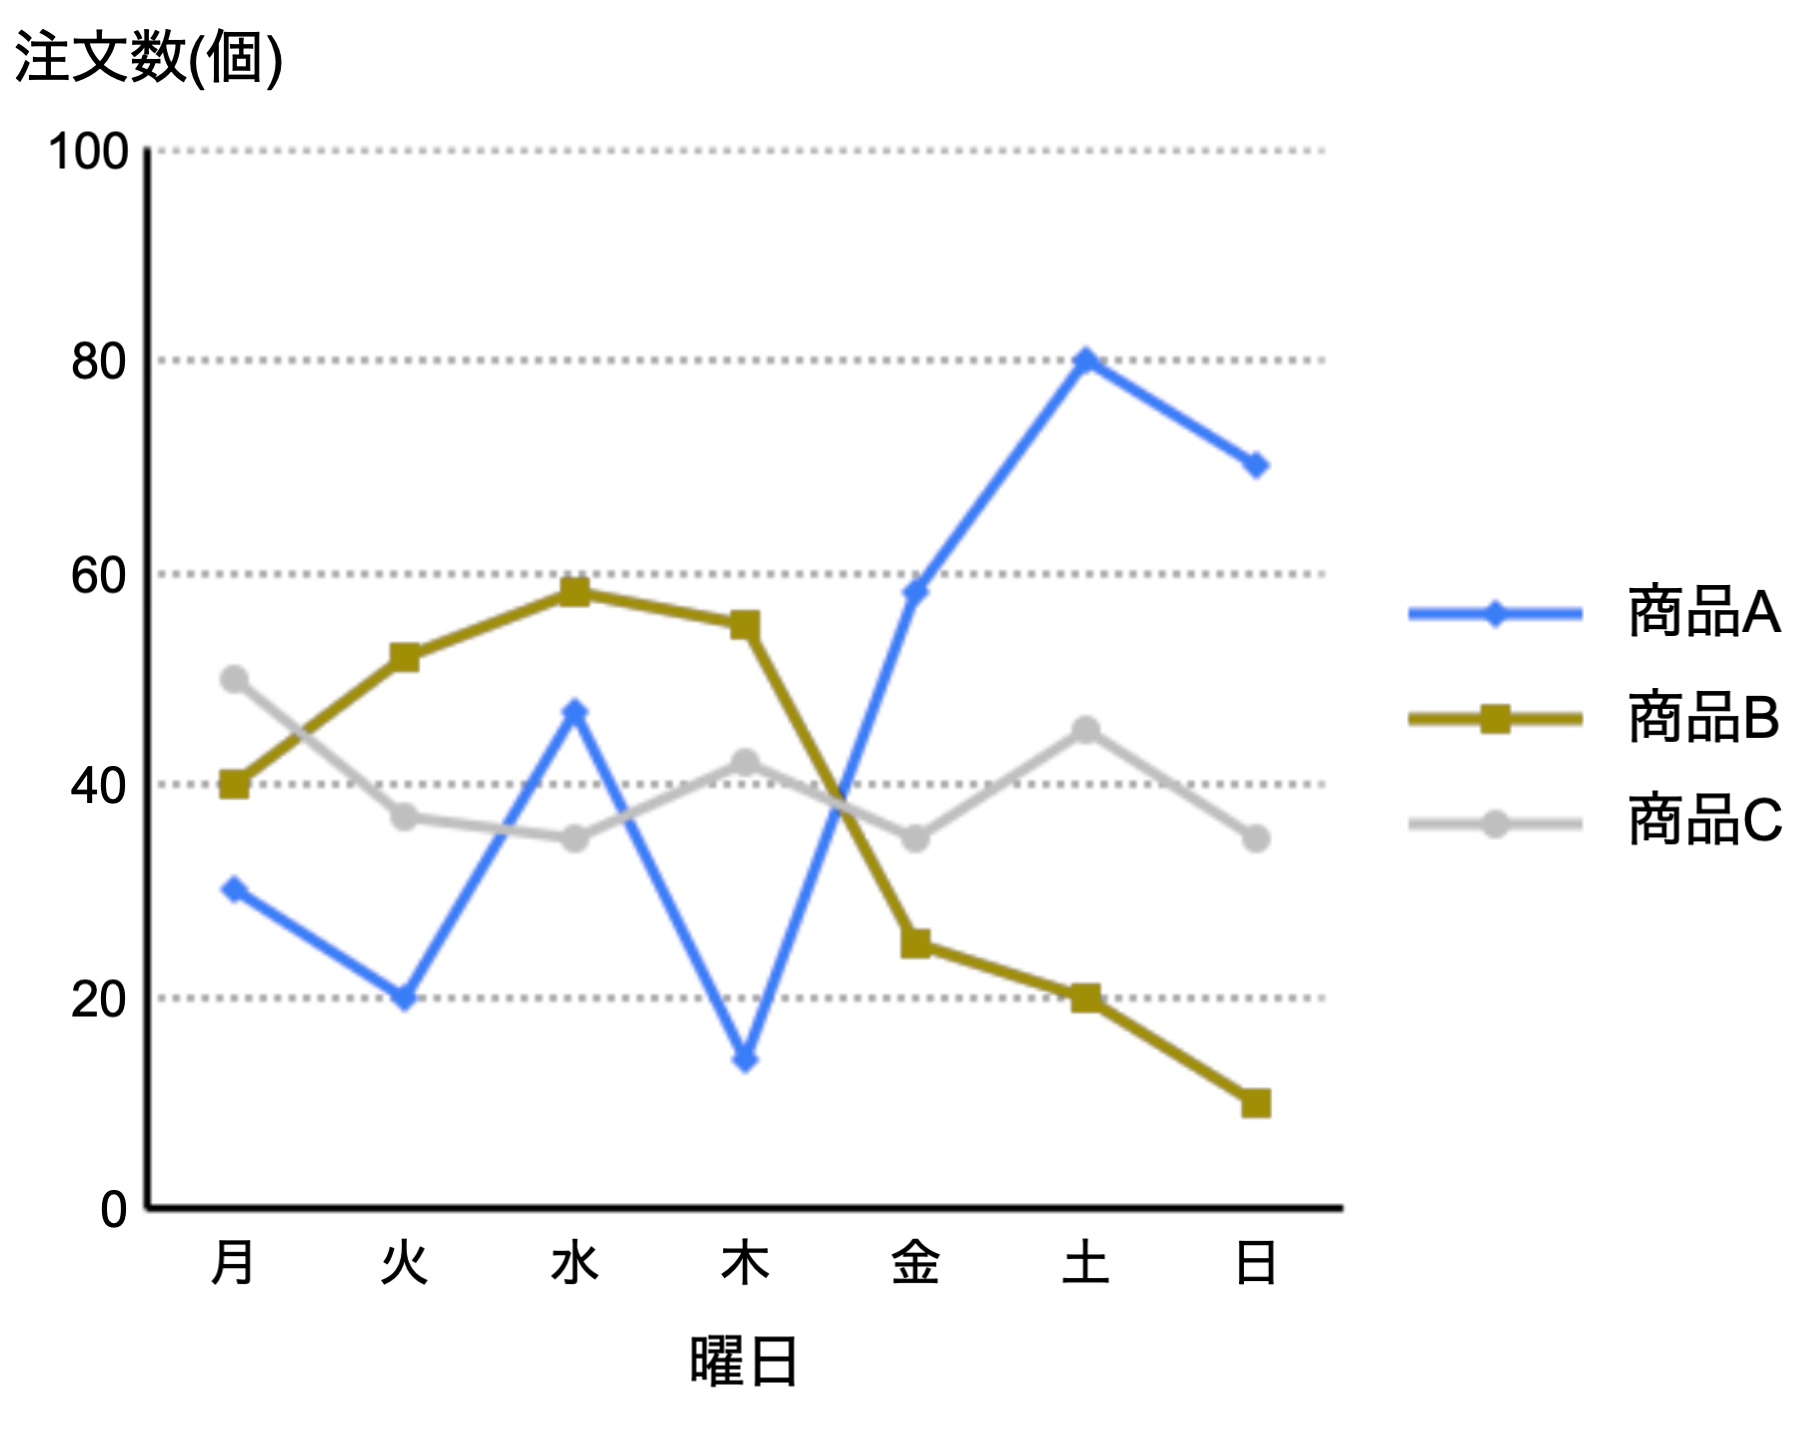
\includegraphics[keepaspectratio,width=\textwidth]{../../10_UniversalDesign/no2_line_RC_D.png}
        \subcaption{改良後(D型)}
    \end{minipage}
    \begin{minipage}[b]{.49\columnwidth}
        \centering
        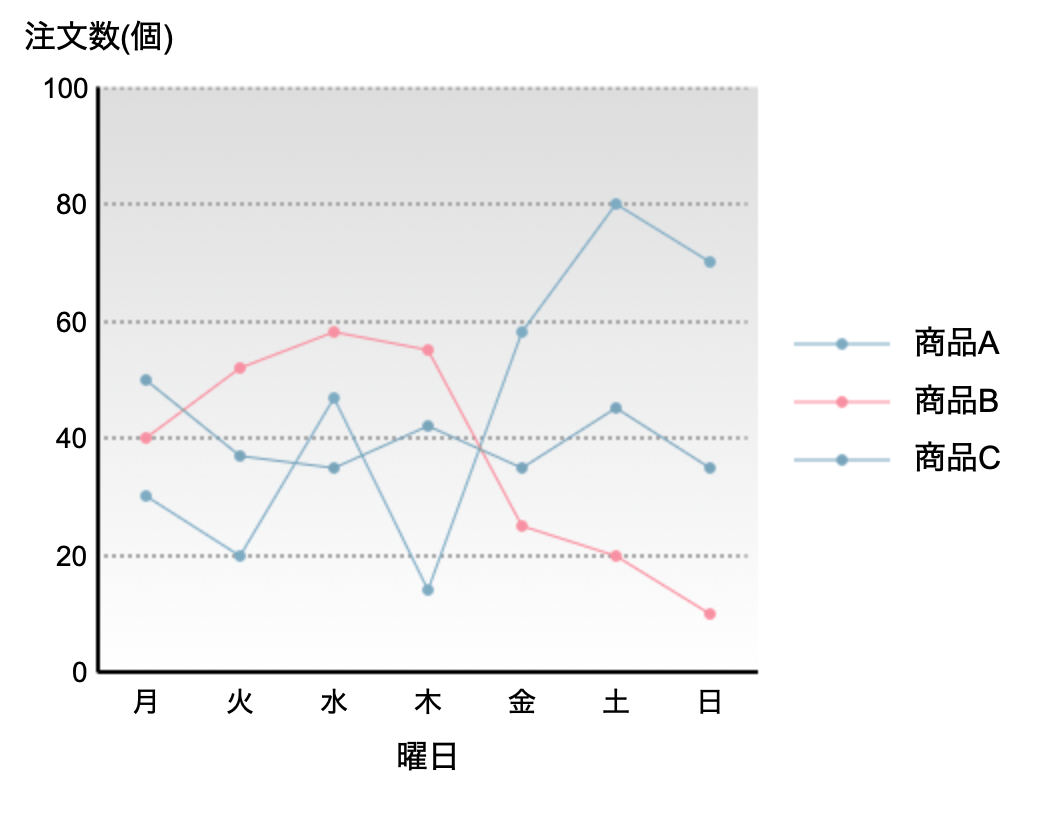
\includegraphics[keepaspectratio,width=\textwidth]{../../10_UniversalDesign/no2_line_CC_T.png}
        \subcaption{改良前(T型)}
    \end{minipage}
    \begin{minipage}[b]{.49\columnwidth}
        \centering
        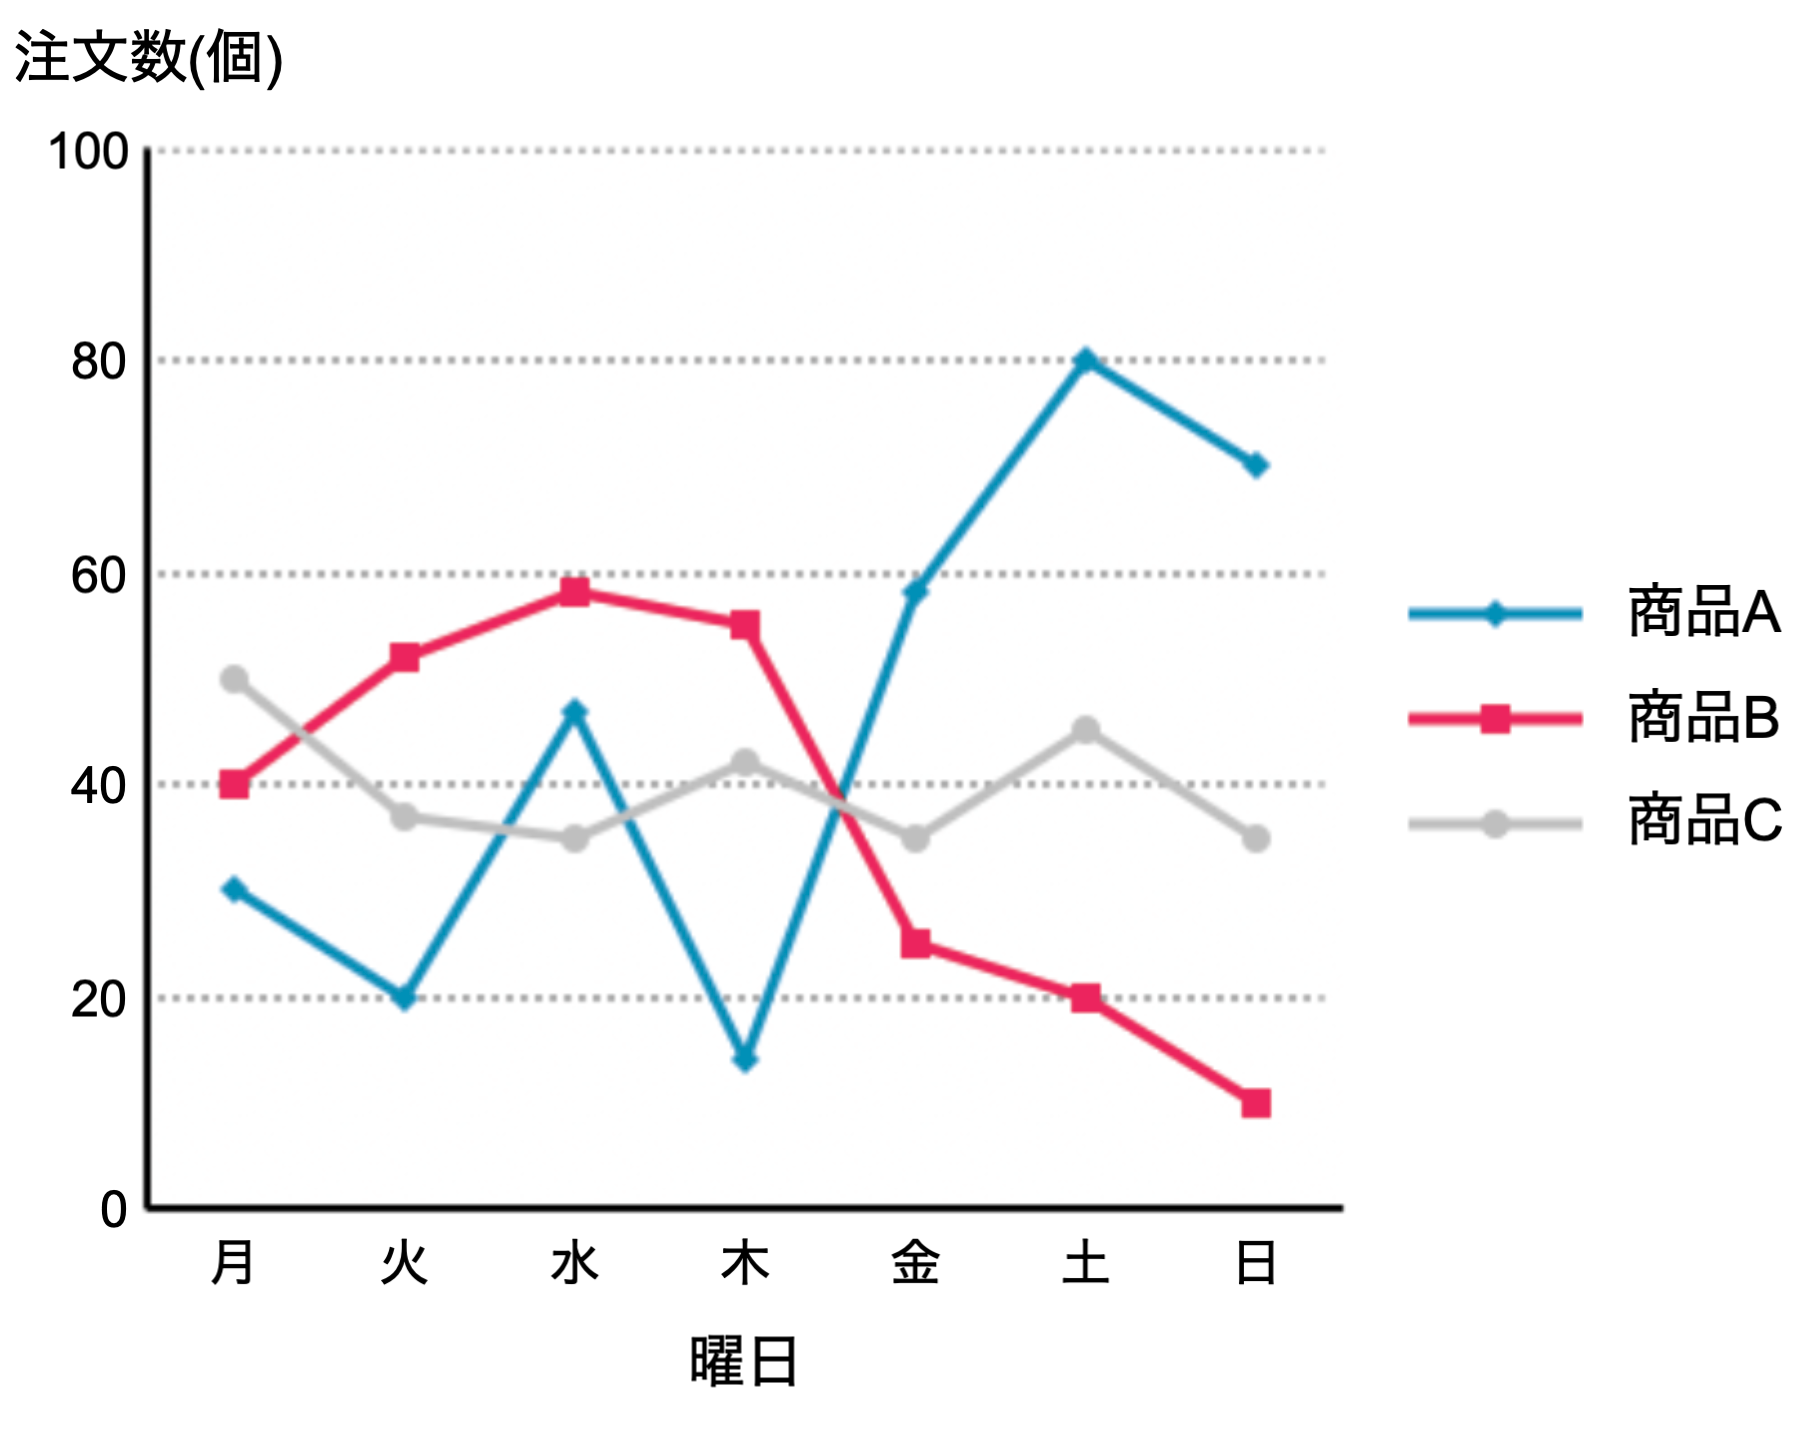
\includegraphics[keepaspectratio,width=\textwidth]{../../10_UniversalDesign/no2_line_RC_T.png}
        \subcaption{改良後(T型)}
    \end{minipage}
    \caption{折れ線グラフ}
\end{figure}
\begin{figure}[H]
    \centering
    \begin{minipage}[b]{.49\columnwidth}
        \centering
        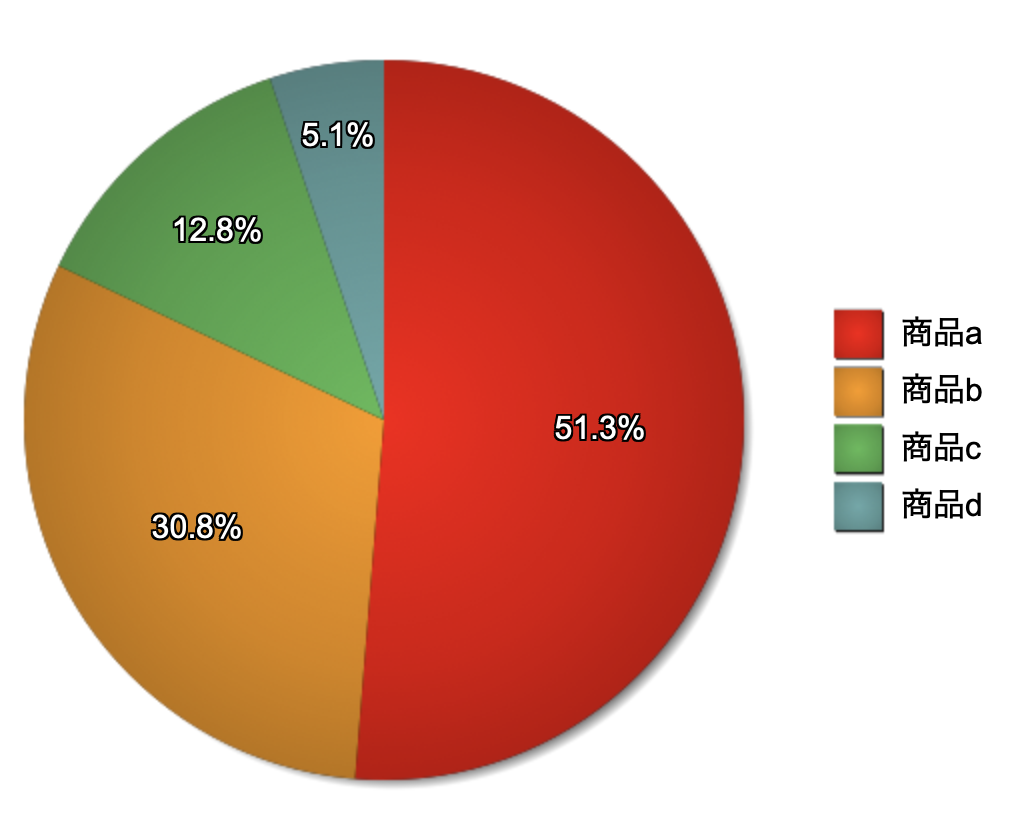
\includegraphics[keepaspectratio,width=\textwidth]{../../10_UniversalDesign/no2_circle_original.png}
        \subcaption{改良前(C型)}
    \end{minipage}
    \begin{minipage}[b]{.49\columnwidth}
        \centering
        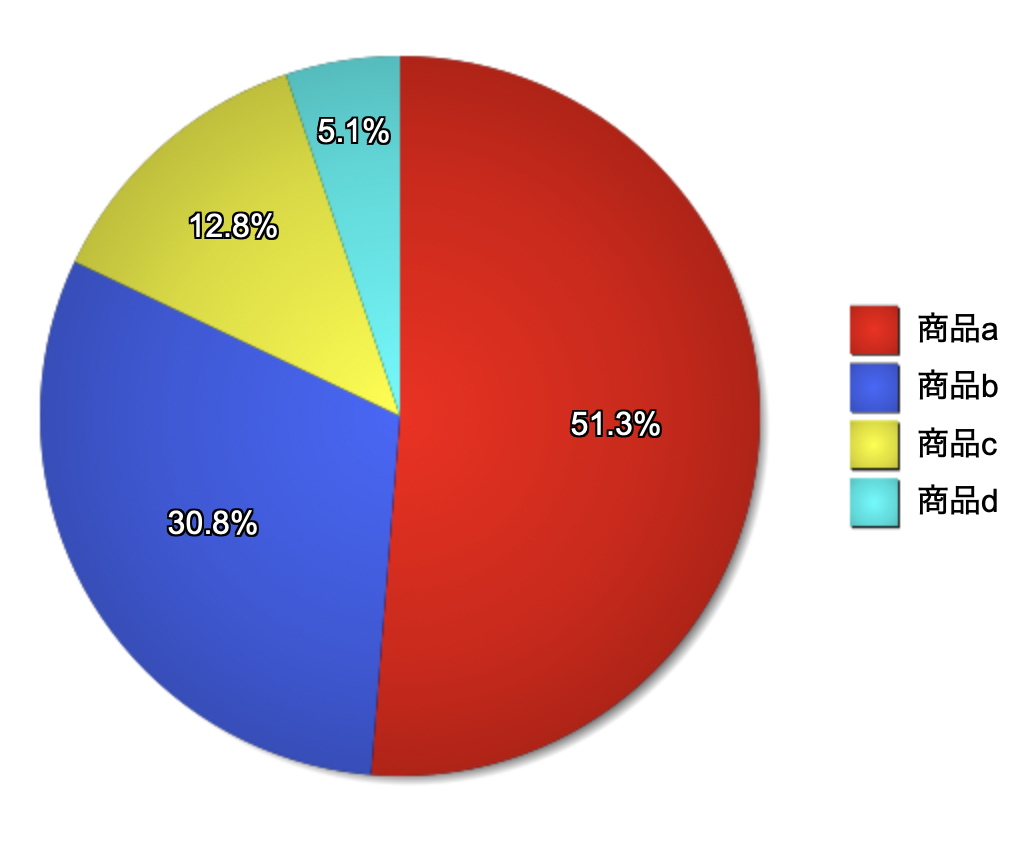
\includegraphics[keepaspectratio,width=\textwidth]{../../10_UniversalDesign/no2_circle_reviced.png}
        \subcaption{改良後(C型)}
    \end{minipage}
    \begin{minipage}[b]{.49\columnwidth}
        \centering
        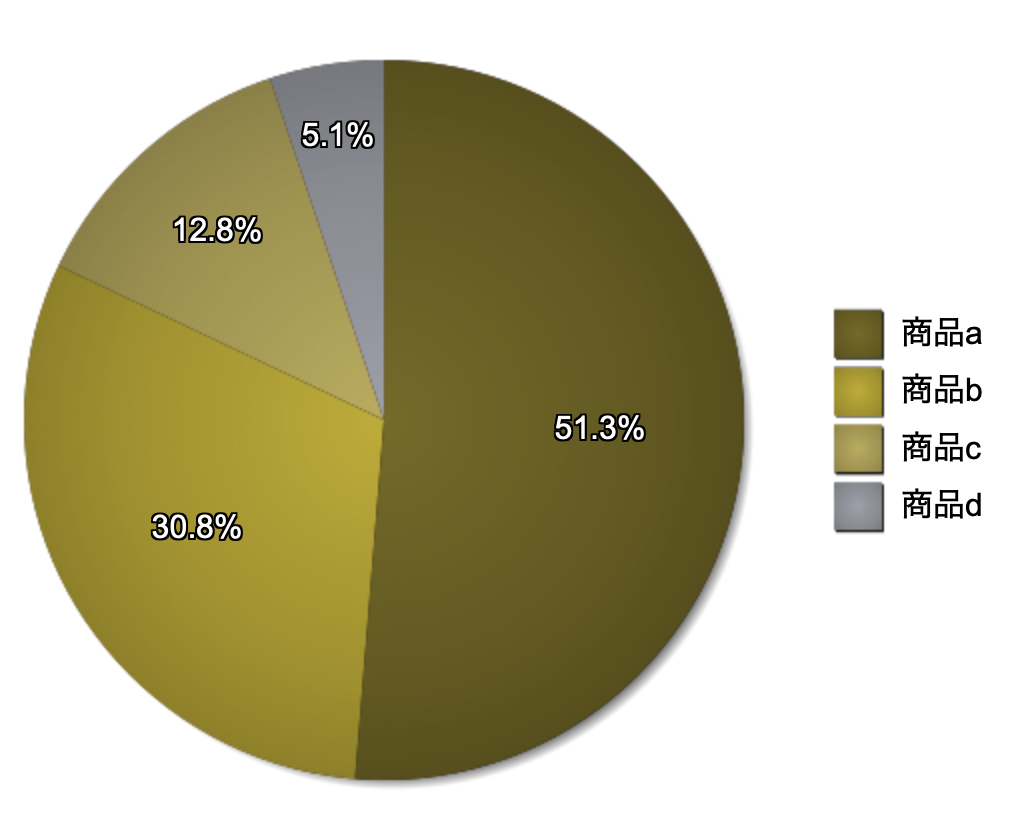
\includegraphics[keepaspectratio,width=\textwidth]{../../10_UniversalDesign/no2_circle_CC_P.png}
        \subcaption{改良前(P型)}
    \end{minipage}
    \begin{minipage}[b]{.49\columnwidth}
        \centering
        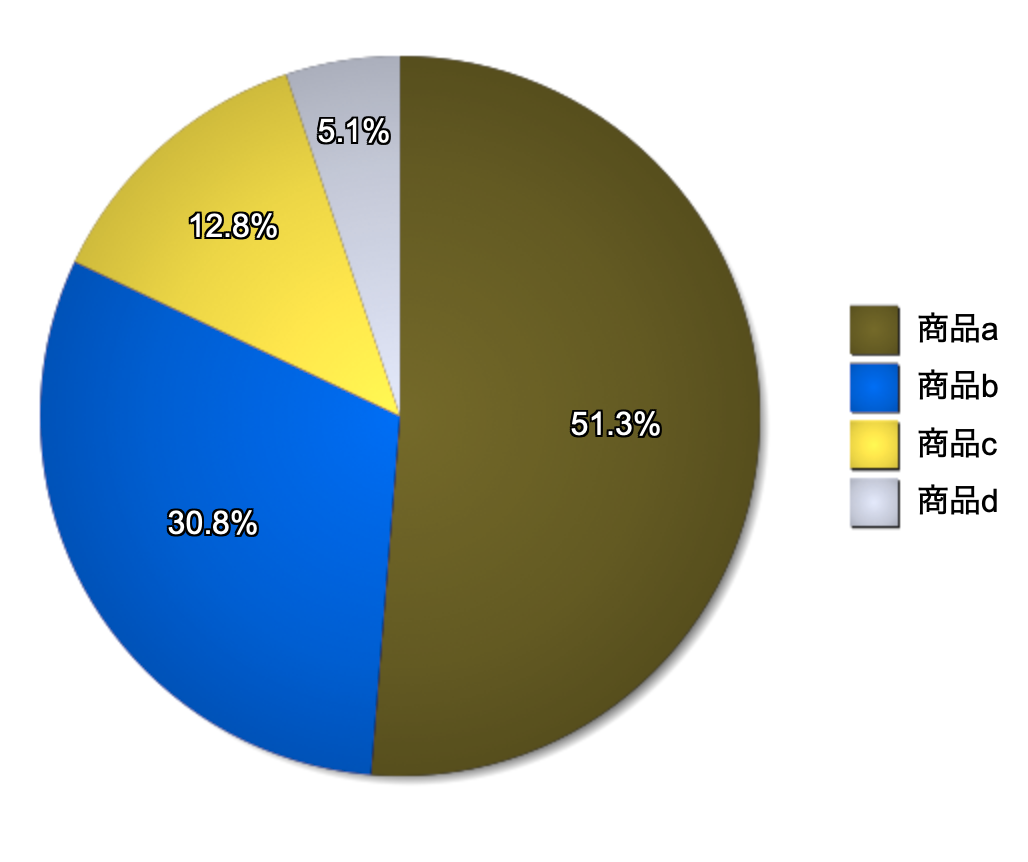
\includegraphics[keepaspectratio,width=\textwidth]{../../10_UniversalDesign/no2_circle_RC_P.png}
        \subcaption{改良後(P型)}
    \end{minipage}
    \begin{minipage}[b]{.49\columnwidth}
        \centering
        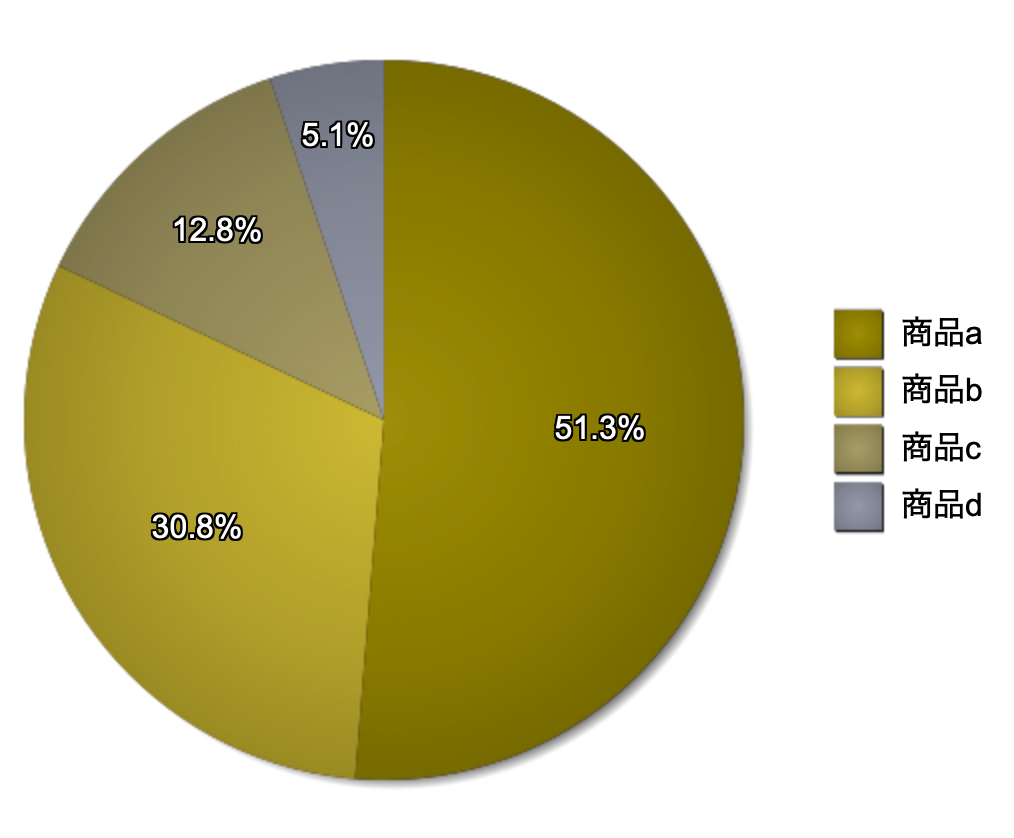
\includegraphics[keepaspectratio,width=\textwidth]{../../10_UniversalDesign/no2_circle_CC_D.png}
        \subcaption{改良前(D型)}
    \end{minipage}
    \begin{minipage}[b]{.49\columnwidth}
        \centering
        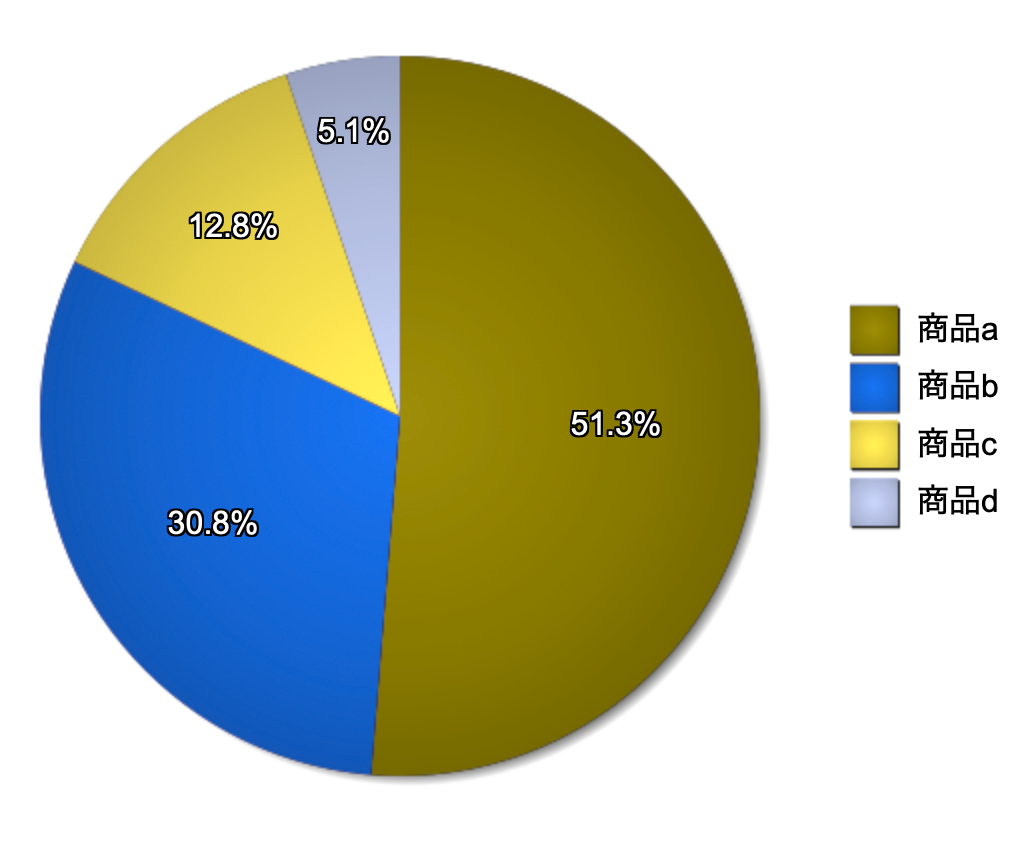
\includegraphics[keepaspectratio,width=\textwidth]{../../10_UniversalDesign/no2_circle_RC_D.png}
        \subcaption{改良後(D型)}
    \end{minipage}
    \begin{minipage}[b]{.49\columnwidth}
        \centering
        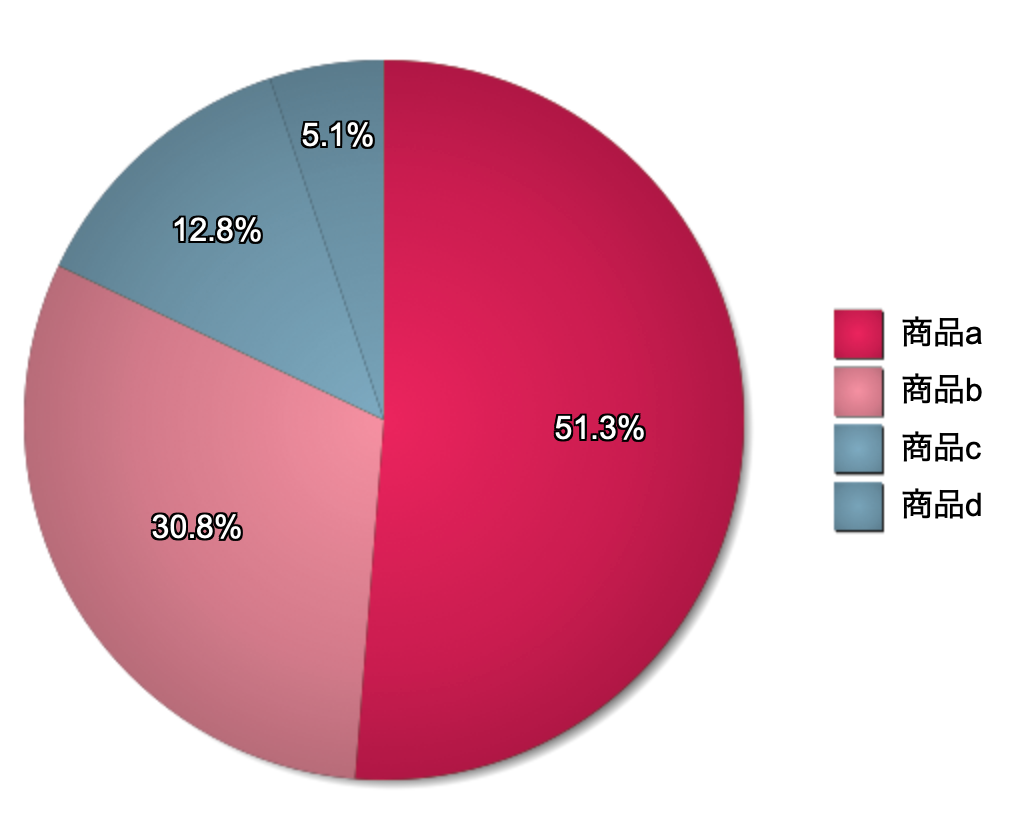
\includegraphics[keepaspectratio,width=\textwidth]{../../10_UniversalDesign/no2_circle_CC_T.png}
        \subcaption{改良前(T型)}
    \end{minipage}
    \begin{minipage}[b]{.49\columnwidth}
        \centering
        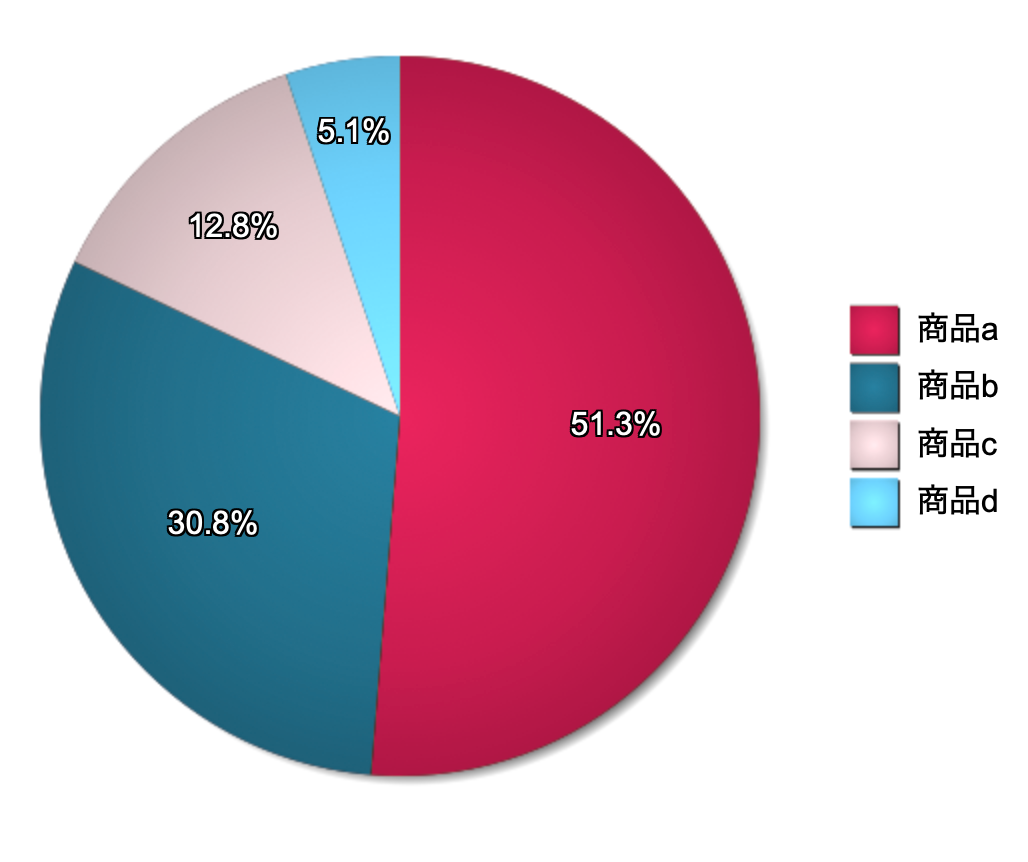
\includegraphics[keepaspectratio,width=\textwidth]{../../10_UniversalDesign/no2_circle_RC_T.png}
        \subcaption{改良後(T型)}
    \end{minipage}
    \caption{円グラフ}
\end{figure}